\begin{figure}[H]
\centering
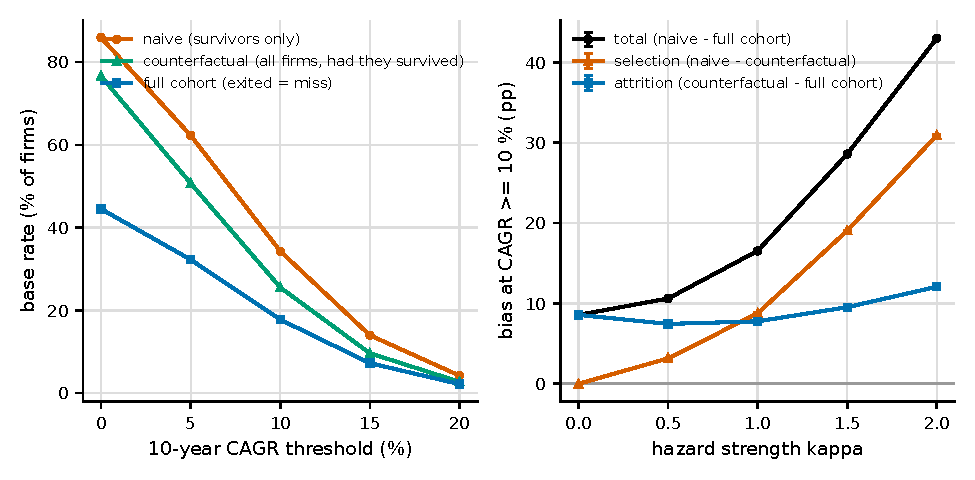
\includegraphics[width=\linewidth]{figures/fig7_survivorship.pdf}
\caption{Survivorship bias in 10-year growth base rates, synthetic universe of 2000 firms (M = 2000 cohorts, base hazard h0 = 0.04). Left: the naive, counterfactual and full-cohort base rates for kappa = 1. Right: at a CAGR threshold of 10\,\%, the total bias and its parts against the hazard strength: selection (survivors are not a random sample) and attrition (exited firms count as misses). Error bars $\pm 1.96$ se (Monte-Carlo noise only, mostly smaller than the markers); the size depends on the assumed hazard.}
\label{fig:fig7_survivorship}
\end{figure}
